 \section{Multimodal Time-Series Forecasting Library: \mmtsf}\label{sec:lib}
In this section, we aim to illustrate the potential benefits of our \model for multimodal TSA by focusing on time-series forecasting (TSF), a fundamental TSA task. TSF involves predicting future events or trends based on historical time-series data. While most existing TSF methods primarily depend on numerical series, we aim to extend these unimodal TSF methods to multimodality. To achieve this, we contribute both formulating the multimodal TSF problem as well as introducing \mmtsf, the first-cut reasonable approach for multimodal TSF.

\subsection{Problem Formulation}


Conventional unimodal TSF models take a numerical series as input and output future values of some or all of its features. Let the input variable of the numerical series be denoted as $\bm{X}\in\mathbb{R}^{l\times d_\mathrm{in}}$, where $l$ is the length of the \textit{lookback window} decided by domain experts and $d_\mathrm{in}$ is the feature dimension at each time step. The output variable of the forecasts generated of \textit{horizon window} length $h$ is denoted as $\bm{Y}\in\mathbb{R}^{h\times d_\mathrm{out}}$, where $d_\mathrm{out}$ is the dimension of targets at each time step.  For the sample at time step $t$, denoted as $(\mathbf{X}_t,\mathbf{Y}_t)$, $\mathbf{X}_{t}\in\bm{X}=\left[\mathbf{x}_{t-l+1}, \mathbf{x}_{t-l+2}, \ldots, \mathbf{x}_{t}\right]$ and $\mathbf{Y}_{t}\in\bm{Y}=\left[\mathbf{y}_{t+1}, \mathbf{y}_{t+2}, \ldots, \mathbf{y}_{t+h}\right]$. Thus, the unimodal TSF model parameterized by $\theta$ is denoted as $f_\theta:\mathcal{X}\rightarrow\mathcal{Y}$.

For multimodal TSF, the input variable of the textual series is also considered, which can be denoted as $\bm{S} \in\mathbb{R}^{k\times d_\mathrm{txt}}$, where $k$ is the lookback window length of the text series, independent of $l$, and $d_\mathrm{txt}$ is the feature dimension of the text. Although the text variable may have inconsistent feature dimensions, we slightly abuse the notation $d_\mathrm{txt}$ here for brevity. Thus, the multimodal TSF model parameterized by $\theta$ is denoted as $g_\theta:\mathcal{X}\times\mathcal{S}\rightarrow\mathcal{Y}$.
\subsection{Pioneering Solution for Multimodal TSF}
\par \noindent \textbf{Multimodal Integration Framework.} We propose a pioneering multimodal integration framework to extend existing unimodal TSF models to their multimodal versions. As illustrated in Figure~\ref{fig:lib}, our framework features an end-to-end pipeline that integrates open-source language models with various TSF models. Numerical and textual series are independently modeled using unimodal TSF models and LLMs with projection layers. These outputs are then combined using a learnable linear weighting mechanism to produce the final prediction. To reduce computational costs, we freeze the LLM parameters and train only the additional projection layers. We employ pooling layers to address the inconsistent dimensions of textual variables. This framework features an end-to-end training manner, with minimal overhead in trainable parameters.
\par \noindent \textbf{Multimodal TSF Library}. Building upon the multimodal dataset \model and integration framework, we present the first multimodal TSF library, named \textbf{\mmtsf}. \mmtsf supports multimodal extensions of over 20 unimodal TSF algorithms through 7 open-source (large) language models, including BERT~\cite{devlin2018bert}, GPT-2~\cite{radford2019language} (Small, Medium, Large, Extra-Large), Llama-2-7B~\cite{touvron2023llama}, and Llama-3-8B\footnote{\url{https://llama.meta.com/llama3}}. We detail the implementations and language models in Appendix~\ref{app:lib}.

\mmtsf is designed for ease of use with \model in multimodal TSA. Additionally, \mmtsf serves as a pilot toolkit for evaluating the multimodal extensibility of existing TSF models.



\begin{figure}[!h]
    \centering
    \begin{minipage}{0.51\linewidth}
        \centering
        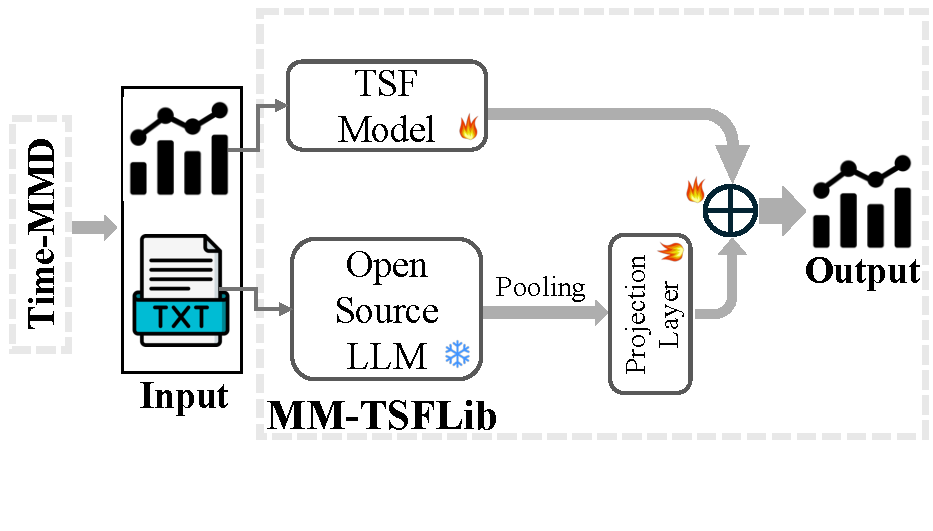
\includegraphics[width = \linewidth]{Figures/lib_overview.pdf}
        \caption{Overall structure of the \mmtsf. \mmtsf uses a model-agnostic multimodal integration framework that independently models numerical and textual series within an end-to-end training manner. \mmtsf slightly increases the number of trainable parameters, balancing effectiveness and efficiency. \label{fig:lib}}
    \end{minipage}
    \hfill
    \begin{minipage}{0.47\linewidth}
        \centering
        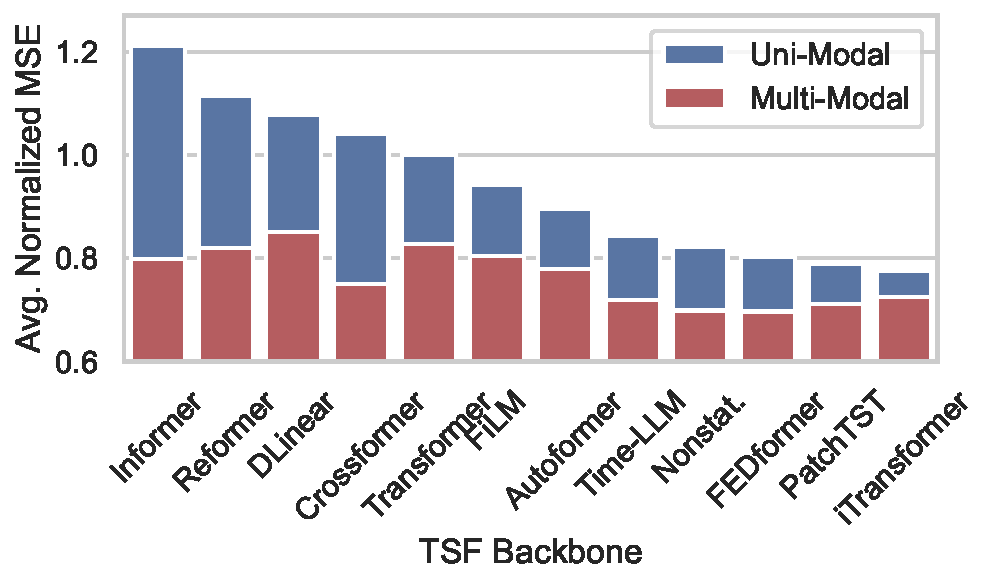
\includegraphics[width = \linewidth]{Figures/boost_model.pdf}
        \caption{Average normalized MSE results for each TSF backbone. Blue areas represent the performance gap between unimodal and multimodal results. The multimodal experiments significantly and consistently outperform corresponding unimodal ones. Detailed results are provided in Appendix \ref{app:detailed_results}\label{subfig:model_boost}} 
    \end{minipage}
\end{figure}
\section{Experiments for Multimodal TSF}
\label{sec:exp}
Based on the constructed \mmtsf, we further conduct comprehensive experiments to demonstrate the superiority of multimodal TSF and the high quality of \model."We further investigate the impact of data domains, horizon window size and the text modeling method.

\subsection{Experimental Setup}
We adhere to the general setups following existing TSF literatures~\cite{wu2021autoformer,wu2023timesnet,nie2022time}. Regarding the horizon window length, we consider a wider range \textbf{from short- to long-term TSF} tasks, with four different lengths for each dataset according to frequency. We conduct TSF tasks on \textbf{all 9 domains of \model}. We employ the widely-adopted mean squared error (MSE) as the evaluation metric. A higher MSE indicates a better performance.

We comprehensively consider \textbf{12 advanced unimodal TSF methods across 4 types} including: (1) Transformer-based: Transformer ~\cite{vaswani2017attention}, Reformer ~\cite{kitaev2020reformer}, Informer ~\cite{zhou2021informer}, Autoformer ~\cite{wu2021autoformer}, Crossformer ~\cite{zhang2022crossformer}, Non-stationary Transformer ~\cite{liu2022non},FEDformer ~\cite{zhou2022fedformer}, iTransformer ~\cite{liu2023itransformer}. (2) MLP-based: DLinear ~\cite{zeng2023transformers}. (3) Agnostic: FiLM ~\cite{zhou2022film}. (4) LLM-based: Time-LLM~\cite{jin2023time}.  Unless otherwise specified, we use GPT-2-Small as the LLM backbone in \mmtsf. We deployed two sets of experiments upon each TSF model, i.e., both unimodal and multimodal versions. More details about experimental setup are provided in Appendix~\ref{app:setup}.
\begin{figure}[t]
    \centering
    \subfloat[\label{subfig:domainBoost}]{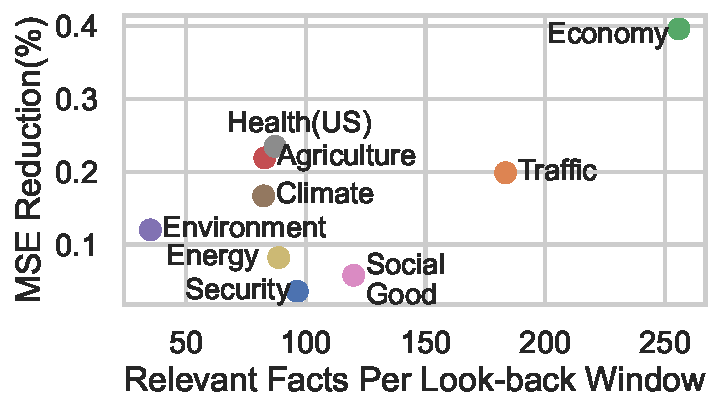
\includegraphics[width = 0.30\linewidth]{Figures/boost_domain_fact.pdf}}
    \hfill
    \subfloat[\label{subfig:backbone}]{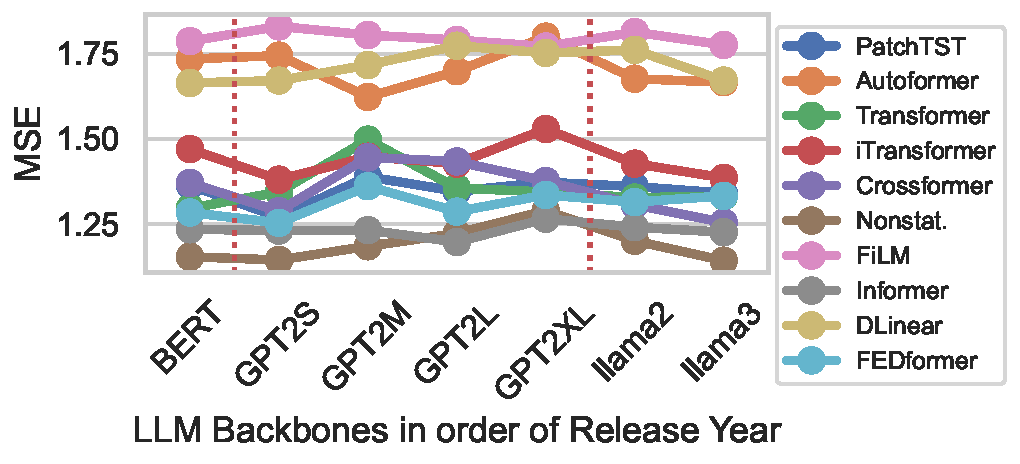
\includegraphics[width = 0.37\linewidth]{Figures/backbone_health.pdf}}
    \hfill
    \subfloat[\label{subfig:predlenBoost}]{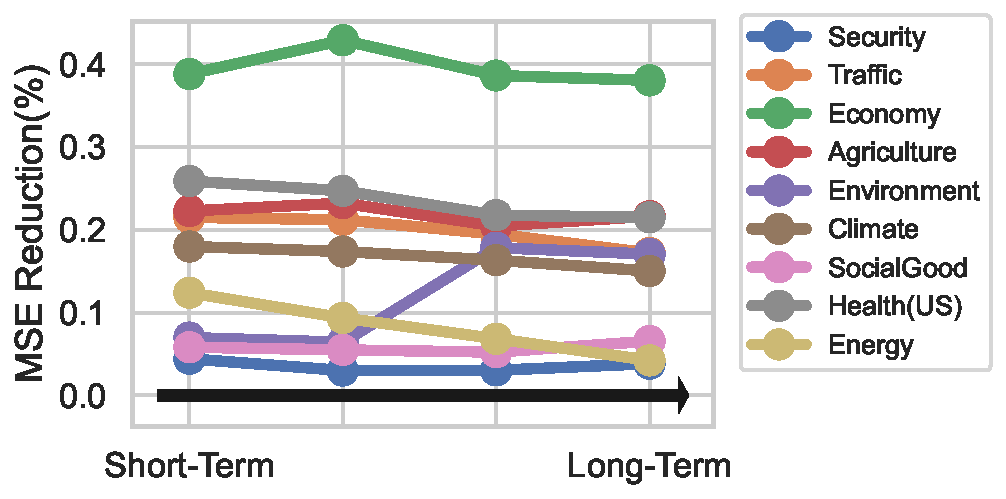
\includegraphics[width = 0.33\linewidth]{Figures/boost_predlen.pdf}}
   \caption{Results of exploratory experiments. (a) Influence of data domains: inherent characteristics and text richness influence performance. (b) Influence of LLM backbones: unclear correlation between multimodal TSF performance and LLM natural language capabilities. (c) Influence of horizon window size: improvements via multimodality are robust to horizon window size.}
   \vspace{-0.2in}
\end{figure}
\subsection{Experimental Results}

Our experiments aim to investigate the following five aspects. Appendix \ref{app:detailed_results} provides detailed results.

\par \noindent \textbf{Effectiveness of multimodal TSF.} Figure \ref{subfig:model_boost} shows average MSE results for corresponding unimodal and multimodal versions of each TSF backbone. The multimodal versions consistently outperform corresponding unimodal versions. As detailed in Appendix \ref{app:detailed_results}, 
the multimodal versions outperformed their unimodal versions in \textbf{95\%} of over 1,000 experiments, reducing the mean squared error by over \textbf{15\%} in average and up to \textbf{40\%} in domains with rich textual data.
Such consistent improvements fully validate the superiority of multimodal TSF and the effectiveness of our proposed multimodal framework in Section~\ref{sec:lib}.

Furthermore, we observe that different TSF backbones benefit from multimodal extension to varying degrees. For example, the originally inferior Informer exhibits strong multimodal performance, which we attribute to its intrinsic design for modeling long-range dependencies that may benefit more from textual cues. 

Additional experiments on text integration approach approaches are provided in Appendix~\ref{app:texti_inte}. We hope these results inspire more advanced multimodal TSF solutions.
\par \noindent \textbf{Quality of \model dataset.} 
Figure~\ref{subfig:model_boost} shows that SOTA unimodal TSF models, such as iTransformer and PatchTST, maintain leading unimodal performance, validating the quality of \model's numerical data. Moreover, multimodal extension consistently and significantly improves performance by incorporating textual data, confirming the quality of \model's textual data.

\par \noindent \textbf{Influence of data domains.} Figure~\ref{subfig:domainBoost} shows the relationship between the relevant fact count and the reduced MSE via multimodal extension for each domain. The scatter plot generally illustrates a positive linear correlation, aligning with the innovation of integrating textual information. Besides, domain characteristics also influence multimodal performance, even with a similar fact count. For example, the security domain, focusing on disasters and emergency grants, exhibits higher unpredictability in the future thus benefits less from the historical textual information. This observation highlights the importance of \model's coverage of 9 diverse domains.

\par \noindent \textbf{Influence of the horizon window size.} Figure~\ref{subfig:predlenBoost} shows the relationship between horizon window size and the average MSE reduction for each domain. 
Overall, the MSE reduction is stable and promising across different horizon window size, from short term to long term. These results demonstrate that the effectiveness of multimodal TSF is robust to different forecast horizon requirements.
\par \noindent \textbf{Influence of the text modeling method.} Firstly, we varied the LLM backbone in \mmtsf and evaluated corresponding multimodal performance on health domain. As shown in Figure~\ref{subfig:backbone}, the choice of LLM backbone does not exhibit a significant correlation with multimodal TSF performance. For the GPT2 series, the scaling law is unclear for multimodal TSF, indicating no clear positive correlation between the parameter scale and TSF performance. Across different LLMs, multimodal TSF performance is relatively similar, even between the advanced Llama-3-8B and the earlier BERT. There might be three possible reasons:
(1) Our proposed multimodal framework, although effective, still does not fully utilize the power of LLMs, particularly by only fine-tuning through projection layers. (2) Existing LLMs, pre-trained for natural language tasks, may not be directly suitable for multimodal TSF. (3) The embedding dimension of BERT is 768, much lower than the 4096 dimension size of Llama-3-8B, thereby makes it easier to fine-tune an effective projection layer with limited training data. 

Although LLMs are currently the mainstream approach for text modeling, they may not be suitable for certain scenarios, such as unfamiliar domains or unsupported languages. Therefore, we introduce Doc2Vec~\cite{le2014distributed} a text embedding model trained from scratch, as an alternative for text modeling. The experimental results on three datasets across four prediction horizons are provided in Table~\ref{tab:TI}. The results show that Doc2Vec is also effective but generally performs worse than BERT. Doc2Vec is further included in our \mmtsf, which will greatly enhance applicability to underrepresented languages and domains. 

We provide additional experiments and discussions on multimodal modeling approaches in Appendix~\ref{app:mma}, including the introduction of attention mechanisms~~\cite{vaswani2017attention} and the use of closed-source LLMs, such as GPT-3.5\footnote{\url{https://platform.openai.com/docs/models/gpt-3-5-turbo}}.

In summary, all these observations suggest that there is significant room for improvement in the methodological research for multimodal TSF.